\documentclass{standalone}

\usepackage{tikz}
    \usetikzlibrary{arrows.meta}
    \usetikzlibrary{calc}
    \usetikzlibrary{decorations.pathmorphing}

\tikzset{
    bluearrow/.style={
        blue!25,
        -{Kite[length=2.5mm]}, 
        line width=0.5mm,},
    greensq/.style={
        black!60,
        fill=black!5, 
        line width=0.5mm,},
    }
    
\begin{document}
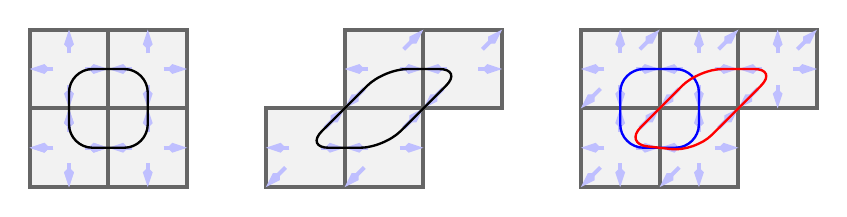
\begin{tikzpicture}
    % \draw[help lines] (0,0) grid (15,3);
    \foreach \x in % green
        {(0,0), (0,1), (1,0), (1,1),% case (A)
         (3,0), (4,0), (4,1), (5,1), % case (C)
         (7,0), (8,0), (7,1), (8,1), (9,1)% case (D6)
        } 
        {\draw[greensq] \x rectangle+(1,1);} 
    % case (A) bound
    \foreach \x in
        {(0,0), (0,1), (1,0), (1,1),} 
        {\draw[bluearrow] \x++(0.3,0.5) -- ++(-0.3,0);
         \draw[bluearrow] \x++(0.7,0.5) -- ++(0.3,0);
         \draw[bluearrow] \x++(0.5,0.3) -- ++(0,-0.3);
         \draw[bluearrow] \x++(0.5,0.7) -- ++(0,0.3);}
    % case (C) bound
    \foreach \x in
        {(3,0), (4,0), (4,1), (5,1)} 
        {\draw[bluearrow] \x++(0.25,0.25) -- ++(-0.25,-0.25);
         \draw[bluearrow] \x++(0.75,0.75) -- ++(.25,0.25);
         \draw[bluearrow] \x++(0.3,0.5) -- ++(-0.3,0);
         \draw[bluearrow] \x++(0.7,0.5) -- ++(0.3,0);}
    % case (D6) bound
    \foreach \x in
        {(7,0), (8,0), (7,1), (8,1), (9,1)} 
        {\draw[bluearrow] \x++(0.25,0.25) -- ++(-0.25,-0.25);
         \draw[bluearrow] \x++(0.75,0.75) -- ++(.25,0.25);
         \draw[bluearrow] \x++(0.3,0.5) -- ++(-0.3,0);
         \draw[bluearrow] \x++(0.7,0.5) -- ++(0.3,0);
         \draw[bluearrow] \x++(0.5,0.3) -- ++(0,-0.3);
         \draw[bluearrow] \x++(0.5,0.7) -- ++(0,0.3);}
    \draw[line width=0.3mm, rounded corners=3mm]
        (0.5,0.5)--(1.5,0.5)--(1.5,1.5)--(0.5,1.5)--cycle
        (3.5,0.5)--(4.5,1.5)--(5.5,1.5)--(4.5,0.5)--cycle;
    \draw[line width=0.3mm, rounded corners=3mm][blue]
        (7.5,0.5)--(8.5,0.5)--(8.5,1.5)--(7.5,1.5)--cycle;
    \draw[line width=0.3mm, rounded corners=3mm,red]
        (7.55,0.55)--(8.5,1.5)--(9.5,1.5)--(8.45,0.45)--cycle;
\end{tikzpicture}
\end{document}